
\documentclass[10pt,journal,onecolumn]{IEEEtran}
\IEEEoverridecommandlockouts
\usepackage[T1]{fontenc}
\usepackage[utf8]{inputenc}
\usepackage{cite}
\usepackage{url}
\usepackage{booktabs}
\usepackage{tabularx}
\usepackage{longtable}
\usepackage{array}
\usepackage{enumitem}
\usepackage{listings}
\usepackage{xcolor}
\usepackage{amsmath,amssymb}
\usepackage{tikz}
\usetikzlibrary{positioning,arrows.meta,fit,shapes.geometric}
\usepackage[hidelinks]{hyperref}
\lstset{basicstyle=\ttfamily\scriptsize,breaklines=true,columns=fullflexible,frame=single}
\linespread{1.18}
\setlist[itemize]{leftmargin=*,itemsep=1pt,topsep=2pt}
\setlist[enumerate]{leftmargin=*,itemsep=1pt,topsep=2pt}
\newcolumntype{Y}{>{\raggedright\arraybackslash}X}
\begin{document}
\title{JPCM-1.0.0 and the Joint Master Control Plane: A Final Protocol, Authority, Evidence, and Attention Architecture for Autonomous Engineering}
\author{Jepson Taylor and OpenAI GPT-5.5 Thinking}
\maketitle
\begin{abstract}
Autonomous coding agents, tool protocols, and multi-agent frameworks can now perform useful engineering work, but they do not by themselves solve the harder problem: how a user safely controls a population of untrusted workers, tools, datastores, memories, and production pathways without drowning in information. This paper defines the Joint Master Control Plane (JMCP) as an assured supervisory control plane for autonomous engineering and defines JPCM-1.0.0, a mandatory, versioned communication protocol for every service that communicates with JMCP. The design treats Model Context Protocol (MCP), Agent2Agent (A2A), coding agents, CI systems, databases, voice surfaces, and dashboards as subordinate interoperability surfaces rather than sovereign authority planes. JPCM specifies signed envelopes, capability leases, service/tool/data cards, work orders, task state machines, evidence bundles, policy receipts, memory proposals, attention packets, voice command candidates, incidents, self-improvement proposals, and automated tool-building workflows. The core doctrine is simple: no JPCM, no trust; no lease, no side effect; no proof, no promotion; no silent high-risk action; and no self-improvement without governed experiment. The result is a critique-hardened architecture for a software-fab operating system that can minimize user attention while maximizing safety, observability, performance, and long-term engineering yield.
\end{abstract}
\begin{IEEEkeywords}
Autonomous agents, control plane, AI safety, software engineering, observability, workflow, protocol design, capability security, evidence, voice interface.
\end{IEEEkeywords}

\section{Introduction}
The next bottleneck in autonomous engineering is not merely model capability. It is control. A coding agent can edit files, run tests, call tools, and propose pull requests. A tool protocol can expose useful capabilities. An agent protocol can allow one agent to discover another. None of these by itself decides which work should exist, which worker should receive authority, which side effects are allowed, what evidence is sufficient, which memories are safe to keep, or when a human should be interrupted. Those decisions require a supervisory control plane.

The Joint Master Control Plane (JMCP) is that control plane. Its job is to let the human rise above low-level operational noise while retaining sovereignty over high-risk decisions. It behaves less like a chat assistant and more like a process-control system for software and knowledge work. It sees all work cells, tasks, tools, agents, repositories, data sources, incidents, evidence, and memory proposals. It should continuously look for bugs, redundant code, security risks, failing CI, stale standards, tool gaps, and bottlenecks. It should also perform brand-new work: research, knowledge compression, repository creation, tool generation, architecture exploration, and governed self-improvement.

This paper finalizes the missing center of gravity from prior JMCP drafts: the protocol. JPCM-1.0.0 is the mandatory communication and task-control standard used by all programs, services, users, tools, agents, voice surfaces, datastores, and adapters. If an action or claim is outside JPCM, it is not authoritative. This is deliberately stricter than ordinary observability or workflow systems because autonomous agents create side effects and can launder untrusted context into privileged action.

\textbf{Contributions.} This paper contributes: (1) a final definition and negative definition of JMCP; (2) a hostile review of failure modes; (3) JPCM-1.0.0 as a versioned protocol with a companion JSON Schema; (4) a task, lease, evidence, and attention model covering all work including self-improvement and automated tool-building; (5) a reference architecture for a Rust/Vite/TypeScript/React implementation; and (6) an extreme future vector toward an autonomous engineering operating system.


\begin{figure}[t]
\centering
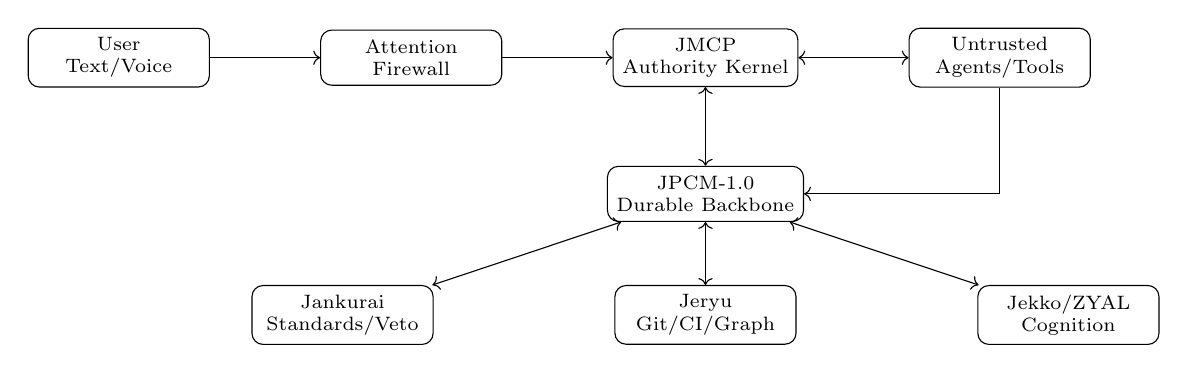
\begin{tikzpicture}[node distance=8mm, every node/.style={font=\scriptsize}, box/.style={draw, rounded corners, align=center, minimum height=7mm, minimum width=23mm}]
\node[box] (user) {User\\Text/Voice};
\node[box, right=14mm of user] (attn) {Attention\\Firewall};
\node[box, right=14mm of attn] (jmcp) {JMCP\\Authority Kernel};
\node[box, below=10mm of jmcp] (bus) {JPCM-1.0\\Durable Backbone};
\node[box, below left=8mm and 22mm of bus] (jank) {Jankurai\\Standards/Veto};
\node[box, below=8mm of bus] (jeryu) {Jeryu\\Git/CI/Graph};
\node[box, below right=8mm and 22mm of bus] (jekko) {Jekko/ZYAL\\Cognition};
\node[box, right=14mm of jmcp] (agents) {Untrusted\\Agents/Tools};
\draw[->] (user) -- (attn); \draw[->] (attn) -- (jmcp); \draw[<->] (jmcp) -- (bus); \draw[<->] (bus) -- (jank); \draw[<->] (bus) -- (jeryu); \draw[<->] (bus) -- (jekko); \draw[<->] (jmcp) -- (agents); \draw[->] (agents) |- (bus);
\end{tikzpicture}
\caption{JMCP centralizes authority and user attention while delegating execution through JPCM. Subordinate systems are useful but not sovereign.}
\label{fig:architecture}
\end{figure}

\section{Hostile Review of the Draft Corpus}
The uploaded V4/V5 corpus was already strong on the idea that JMCP should be an authority-and-evidence layer rather than a mere dashboard. The remaining weakness was finality: many sections described what the protocol should do, but did not make the protocol sufficiently machine-checkable. The JSON schemas were useful envelope sketches, but did not define the full object model for work orders, tasks, leases, evidence, service cards, data cards, attention packets, voice turns, memory proposals, self-improvement proposals, and tool-building proposals.

A second weakness was distributed-systems realism. A control plane cannot assume exactly-once delivery, perfect ordering, or reliable worker behavior. Duplicate events, lost acknowledgments, stream retention limits, partial partitions, poisoned messages, incompatible schema versions, replay gaps, and exhausted consumers are normal operating conditions. The final design therefore assumes at-least-once delivery and requires idempotency, dedupe keys, ordering keys, replay, poison queues, and backpressure semantics.

A third weakness was the user-attention model. The drafts correctly wanted to protect the user from information overload, but the system must also protect against false quiet. A system that suppresses important decisions is more dangerous than a noisy dashboard because the user may believe silence means safety. The final design treats attention as a safety-critical subsystem with explicit attention classes, decision packets, drill-down, and false-quiet tests.

A fourth weakness was self-improvement. The drafts said JMCP should always improve, but a control plane that changes its own memory, policy, scheduler, prompts, tools, or protocol is a high-risk system. The final design makes self-improvement a first-class task family whose schema forbids self-promotion. Every self-improvement proposal requires a hypothesis, guardrails, evaluation plan, rollback plan, and risk tier.

\section{What JMCP Is and Is Not}
JMCP is an assured supervisory control plane for autonomous engineering. It owns authority, work definition, evidence promotion, observability, memory governance, tool/data awareness, and user attention. It is the primary interface for text and voice interaction. It is responsible for deciding what should happen, what can happen safely, which worker should do it, what evidence is required, and what the user should see.

JMCP is not a chatbot, not an MCP host, not an A2A router, not a CI replacement, not a log aggregator, not a generic workflow engine, not a model router, and not a dashboard. It may include all of these as subordinate components or adapters. The distinction matters because interoperability is not authority. MCP standardizes how LLM applications integrate with resources, tools, prompts, sampling, roots, and elicitation \cite{mcp}. A2A standardizes agent discovery, tasks, messages, artifacts, streaming, push notifications, and agent cards \cite{a2a}. JMCP uses these protocols but does not delegate sovereignty to them.

OpenClaw is important prior art because it frames a long-lived gateway that owns many messaging surfaces and validates typed WebSocket frames \cite{openclaw}. JMCP borrows the gateway intuition but hardens it into a process-control kernel for untrusted multi-agent engineering. Where a gateway can assume a relatively local trust perimeter, JMCP assumes hostile workers, hostile documents, poisoned tools, compromised dependencies, and ambiguous user commands.

\section{Design Laws}
The final design is governed by ten laws.
\begin{enumerate}
\item No JPCM, no trust.
\item No lease, no side effect.
\item No proof, no promotion.
\item No silent high-risk action.
\item No ambient trust in agents.
\item No memory without provenance.
\item No self-improvement without experiment.
\item No attention spam.
\item No private side channels.
\item No exactly-once fantasy.
\end{enumerate}
These laws are intentionally operational. They can be turned into conformance tests. For example, a Git adapter that accepts a branch write without a valid lease fails the lease law. A tool that publishes a result without artifact digests fails the evidence law. A voice gateway that allows a destructive command without confirmation fails the attention law.

\section{Related Work and Gap}
MCP, A2A, OpenAI Agents SDK, Claude Code, LangGraph, AutoGen, OpenHands, SWE-agent, and SWE-bench represent a rapidly maturing agentic ecosystem \cite{mcp,a2a,openaiagents,openaicodex,claudecode,langgraph,autogen,openhands,sweagent,swebench}. They are valuable, but they are not sufficient for a sovereign control plane. Agent frameworks generally help build agents, route models, call tools, or maintain workflow state. They do not define a universal authority, evidence, attention, and memory contract for every service in an engineering environment.

Recent MCP security work is especially relevant. Analyses of MCP identify protocol-level risks such as missing capability attestation, prompt injection, implicit trust propagation, tool poisoning, and inadequate client-side validation \cite{mcpbreak,smcp,mcptm}. These findings strengthen the JMCP thesis: tool interoperability without independent authority is unsafe. JPCM therefore treats MCP metadata as untrusted input and requires leases and evidence at the adapter boundary.

The software supply-chain literature contributes provenance, build integrity, signing, and attestation patterns. SLSA, Sigstore, and in-toto show how artifacts can carry verifiable provenance \cite{slsa,sigstore,intoto}. CloudEvents, JSON Schema, JWS, RFC 9457, and OpenTelemetry provide useful primitives for event envelopes, schema validation, signing, error semantics, and telemetry \cite{cloudevents,jsonschema,rfc7515,rfc9457,opentelemetry}. Classic distributed-systems work reminds us that ordering, clocks, consensus, and partitions are design constraints, not implementation details \cite{lamport,paxos,raft,cap}.

\section{Threat Model}
JMCP assumes that agents hallucinate, tools lie, dependencies change, data stores contain malicious content, memory can be poisoned, voice can be misheard, users can be tired, and adapters can be compromised. It also assumes economic attacks: a worker can spend too much money, consume too many tokens, trigger too many CI runs, or spawn useless recursive work. The attacker may be an external adversary, a malicious package, a compromised MCP server, a low-quality agent, a poisoned document, a mistaken user, or a subtle optimization pressure.

The most dangerous failures are authority collapse, confused-deputy routing, evidence theater, memory poisoning, false quiet, sandbox escape, supply-chain compromise, protocol drift, cost explosions, and ungoverned self-improvement. JMCP does not eliminate these risks by trusting a better model. It constrains them with leases, sandboxing, evidence requirements, independent verification, typed events, policy receipts, attention decisions, and rollback.

\section{Reference Architecture}
The architecture has nine planes: authority, communication, workflow, evidence, observability, tool/data awareness, memory/experience, user, and integration. The Authority Plane issues leases and policy decisions. The Communication Plane validates and routes JPCM events. The Workflow Plane owns intents, work orders, task DAGs, scheduling, cancellation, and rollback. The Evidence Plane verifies claims and controls promotion. The Observability Plane reconstructs what happened. The Tool/Data Awareness Plane knows available and missing capabilities. The Memory Plane accepts or rejects lessons. The User Plane handles text, voice, cockpit views, and decision packets. The Integration Plane connects Jankurai, Jeryu, Jekko/ZYAL, MCP, A2A, CI, and external agents.

Jankurai is the standards, lessons, proof-lane, and veto system. Jeryu is the code, CI, Git, and graph reality system. Jekko/ZYAL is the native cognition and workflow substrate. External agents such as Codex or Claude are untrusted workers. This split preserves one critical invariant: execution is delegated, but authority remains centralized.


\begin{figure}[t]
\centering
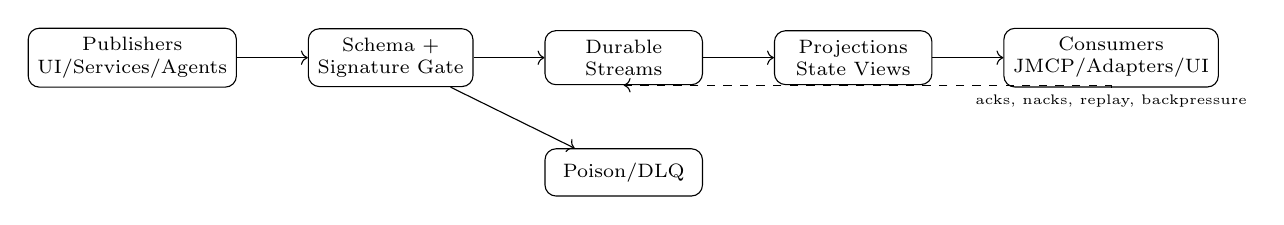
\begin{tikzpicture}[node distance=7mm, every node/.style={font=\scriptsize}, box/.style={draw, rounded corners, align=center, minimum height=6mm, minimum width=20mm}]
\node[box] (pub) {Publishers\\UI/Services/Agents};
\node[box, right=9mm of pub] (val) {Schema +\\Signature Gate};
\node[box, right=9mm of val] (stream) {Durable\\Streams};
\node[box, below=8mm of stream] (dlq) {Poison/DLQ};
\node[box, right=9mm of stream] (proj) {Projections\\State Views};
\node[box, right=9mm of proj] (cons) {Consumers\\JMCP/Adapters/UI};
\draw[->] (pub)--(val); \draw[->] (val)--(stream); \draw[->] (stream)--(proj); \draw[->] (proj)--(cons); \draw[->] (val)--(dlq); \draw[->, dashed] (cons.south) |- node[below, font=\tiny]{acks, nacks, replay, backpressure} (stream.south);
\end{tikzpicture}
\caption{JPCM backbone: validation before persistence, replayable streams, projections, and poison queues.}
\label{fig:backbone}
\end{figure}

\section{JPCM-1.0.0 Protocol}
JPCM-1.0.0 is a signed envelope protocol and task-control grammar. The companion JSON Schema is normative. The envelope includes version, id, type, subject, time, source, producer, tenant, cell, trace context, correlation, actor, authority context, risk context, privacy context, delivery context, schema reference, payload hash, signature, and payload.

\subsection{Envelope Semantics}
The envelope is immutable. Corrections are new messages with causation references. Producers sign canonicalized envelopes. Payloads are hashed. Consumers validate schema, signature, version, and authority before acting. Side effects use idempotency keys. Ordering keys are explicit. Events are durable unless marked ephemeral.

\subsection{Message Families}
JPCM includes service health, user intent, text, voice, work order, task, lease, context, tool, data, evidence, promotion, rollback, policy, memory, technology scouting, tool building, self-improvement, incident, and audit families. The breadth is deliberate: every meaningful action must have a common grammar.

\subsection{Transports}
JPCM is transport-neutral but not semantics-neutral. The canonical deployment uses NATS JetStream for durable streams and work queues, gRPC for low-latency internal calls, WebSocket/SSE for UI updates, WebRTC for voice, and adapters for MCP, A2A, CLIs, databases, and external APIs. JetStream-style persistence and replay are useful because a control plane must reconstruct past decisions and task state \cite{nats}. Temporal-like durable execution concepts are relevant for long-running workflows but do not replace protocol-level authority \cite{temporal}.

\subsection{Versioning}
Additive fields may be introduced in minor-compatible schemas. Removing fields, changing field meaning, expanding authority, or changing task/evidence state semantics requires a major version. Services publish supported versions in ServiceCards. Bridges must preserve causality, authority, and evidence semantics.


\begin{figure}[t]
\centering
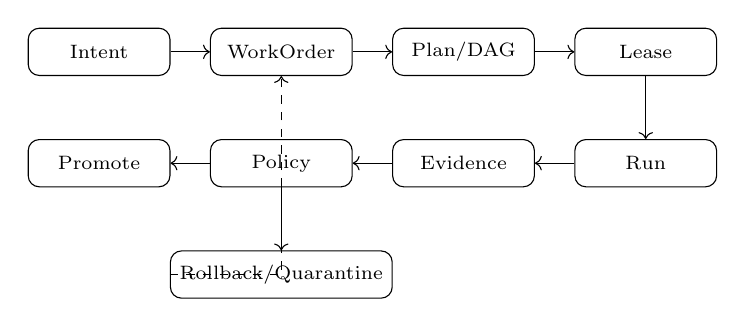
\begin{tikzpicture}[node distance=5mm, every node/.style={font=\scriptsize}, st/.style={draw, rounded corners, minimum width=18mm, minimum height=6mm, align=center}]
\node[st] (intent) {Intent};
\node[st, right=5mm of intent] (wo) {WorkOrder};
\node[st, right=5mm of wo] (plan) {Plan/DAG};
\node[st, right=5mm of plan] (lease) {Lease};
\node[st, below=8mm of lease] (run) {Run};
\node[st, left=5mm of run] (evi) {Evidence};
\node[st, left=5mm of evi] (policy) {Policy};
\node[st, left=5mm of policy] (promote) {Promote};
\node[st, below=8mm of policy] (rollback) {Rollback/Quarantine};
\draw[->] (intent)--(wo); \draw[->] (wo)--(plan); \draw[->] (plan)--(lease); \draw[->] (lease)--(run); \draw[->] (run)--(evi); \draw[->] (evi)--(policy); \draw[->] (policy)--(promote); \draw[->] (policy)--(rollback); \draw[->, dashed] (rollback.west) -| (wo.south);
\end{tikzpicture}
\caption{Canonical task flow. No task can be promoted without leases, evidence, and policy.}
\label{fig:task}
\end{figure}

\section{Task and Workflow Model}
All work follows the hierarchy Intent $\rightarrow$ WorkOrder $\rightarrow$ Task DAG $\rightarrow$ Tool Calls / Agent Runs $\rightarrow$ Evidence $\rightarrow$ Promotion or Rollback. A user may submit a minimal instruction, but JMCP must expand it into scoped work before granting authority.

Work orders include title, intent, task type, risk tier, autonomy tier, state, owner, acceptance criteria, non-goals, budgets, required evidence, rollback plan, and attention policy. Tasks include dependencies, assignee, leases, evidence, progress, deadlines, and rollback links. This makes routine automation and ambitious autonomous work part of the same controlled system.

The task taxonomy includes research, concept search, knowledge compression, architecture design, repository creation, feature implementation, bug hunting, bug fixing, refactoring, deduplication, performance, security review, vulnerability fixes, dependency updates, CI fixes, tests, documentation, release, deployment, data migration, incident response, root cause analysis, tool building, tool qualification, model evaluation, policy update, protocol update, self-improvement, memory maintenance, UX review, voice flow, cost optimization, compliance review, and code-graph analysis.

\section{Capability Leases}
A capability lease is a non-transferable, revocable, scoped permission. It is not a prompt instruction. It is checked at the adapter boundary immediately before action. A lease includes issuer, recipient, validity window, scopes, risk tier, budgets, constraints, revocation subject, and renewal policy.

Lease scopes are resource-specific: repository, branch, file, directory, database, table, bucket, object, API, tool, model, secret, CI system, cloud account, UI, voice session, control plane, memory store, knowledge graph, and network. This prevents confused-deputy escalation. A read lease does not imply write. A branch-write lease does not imply merge. A tool-execute lease does not imply network egress. A self-improvement proposal lease does not imply self-promotion.

\section{Evidence and Promotion}
Evidence bundles transform agent claims into verifiable control-plane facts. A bundle contains claims, artifacts, digests, verifiers, quality scores, provenance, and policy receipts. Evidence classes include unit tests, integration tests, end-to-end tests, static analysis, security scans, type checks, lint, build, benchmark, diff, review, policy receipt, provenance, attestation, replay, screenshot, human approval, runtime trace, rollback plan, data lineage, and cost receipt.

Promotion requires acceptance criteria, required evidence, verifier independence when risk demands it, artifact digests, policy allowance, Jankurai standards/veto success for code quality, Jeryu CI/Git/graph consistency, rollback plan, and user decision when required. Conflicting evidence blocks promotion. It does not become a weighted average.

\section{Policy, Veto, and Waiver}
JMCP uses policy engines for machine decisions and reserves vetoes for high-confidence blockers. Policies evaluate actor, lease, risk, privacy, task type, evidence, service trust, cost, and user preferences. A policy decision returns allow, deny, veto, require-human, require-more-evidence, quarantine, or waive. Decisions are recorded as receipts. Waivers are explicit, scoped, expiring, and auditable.

OPA/Rego or Cedar-style policies are appropriate implementation choices because they separate policy logic from application code \cite{opa}. However, policy engines are not the control plane. They produce decisions; JMCP manages their lifecycle, evidence, versioning, and incident review.


\begin{figure}[t]
\centering
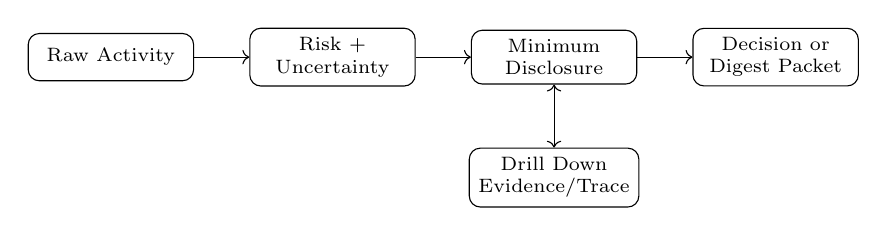
\begin{tikzpicture}[node distance=7mm, every node/.style={font=\scriptsize}, box/.style={draw, rounded corners, align=center, minimum height=6mm, minimum width=21mm}]
\node[box] (raw) {Raw Activity};
\node[box, right=7mm of raw] (risk) {Risk +\\Uncertainty};
\node[box, right=7mm of risk] (min) {Minimum\\Disclosure};
\node[box, right=7mm of min] (packet) {Decision or\\Digest Packet};
\node[box, below=8mm of min] (drill) {Drill Down\\Evidence/Trace};
\draw[->] (raw)--(risk); \draw[->] (risk)--(min); \draw[->] (min)--(packet); \draw[<->] (min)--(drill);
\end{tikzpicture}
\caption{The attention firewall hides routine detail but preserves drill-down and escalates real decisions.}
\label{fig:attention}
\end{figure}

\section{User Attention and Minimal Disclosure}
The user should see the bare minimum needed for judgment. Attention classes are silent, digest, notify, decision, and break-glass. Silent events remain drillable. Digest events become summaries. Notify events require awareness but not action. Decision events require a choice. Break-glass events interrupt.

A decision packet includes summary, why-now, recommended action, options, risk delta, evidence references, deadline, and drill-down. It should not dump raw logs or agent transcripts unless requested. Progressive drill-down moves from summary to evidence, task DAG, tool calls, traces, logs, and artifacts. The system must evaluate false quiet: scenarios where the attention filter would hide decisions users later consider important.

\section{Text and Voice}
Text is the default canonical channel. Voice is a useful realtime interface, but it is untrusted until normalized. A voice segment becomes a command candidate only after transcription, confidence scoring, intent normalization, risk scoring, and policy checks. High-risk voice commands require confirmation, preferably with a text-visible decision card. Voice biometrics cannot bypass leases or policy. Barge-in stop publishes cancellation or pause intent.

Voice support matters because JMCP is the primary interface. A user should be able to ask, ``what is blocking the release?'' or ``clean up the redundant code in this repo,'' and JMCP should answer or act. But the system must never treat casual, ambiguous, or misheard voice as authority for destructive operations.

\section{Tool and Data Awareness}
JMCP is 100\% tool and data aware in the practical sense that every approved service, tool, model, data store, dataset, adapter, CI lane, repository, and evidence verifier has a card in the inventory. ToolCards define schemas, side effects, risk, leases, dry-run support, rollback support, conformance, and status. DataCards define sensitivity, access patterns, retention, lineage, freshness, and quality.

This inventory enables build-vs-buy decisions. JMCP can notice a repeated manual diagnostic task and propose building a tool. It can notice a stale verifier and propose replacement. It can discover a new model or protocol and route a technology scout task. It can retire an unsafe adapter. It can detect that a tool is globally useful and push it to Jankurai after proof.

\section{Automated Tool Building}
Automated tool building is a first-class work type. It begins with a \texttt{technology.gap.detected} or \texttt{technology.build.proposal} event. JMCP defines the problem, expected value, risk, acceptance tests, promotion path, and rollback plan. It builds in a sandbox, generates documentation, executes tests, runs security scans, checks conformance, and registers a probationary ToolCard. The tool earns broader leases only after measured value and clean evidence.

This loop is how JMCP becomes more powerful without becoming reckless. It can continuously create small high-leverage tools: duplicate-code detectors, repo-specific migration helpers, policy linters, graph analyzers, incident summarizers, evidence verifiers, performance profilers, and adapter hardening tests.

\section{Memory and Internal Experience}
JMCP needs an internal stream of experience. That stream should not be confused with private chain-of-thought or unreviewed intuition. It is an event-sourced record of observations, decisions, failures, lessons, and hypotheses. Memories enter through proposals and may be accepted, rejected, compacted, tombstoned, quarantined, or expired.

Global memory requires stronger proof than project memory. A lesson learned in one repository may be harmful in another if overgeneralized. Jankurai should receive cross-repo standards and reusable negative examples only when evidence supports generalization. Memory poisoning is treated as a security incident.

\section{Self-Improvement Governor}
JMCP should always improve. It should improve standards, workflows, routing, memory, evidence verifiers, tools, UI, and protocol. But self-improvement is dangerous because the controller is changing the controller. Therefore, a self-improvement proposal includes target subsystem, hypothesis, change type, guardrails, evaluation plan, rollback plan, risk tier, and human approval requirement. The schema sets \texttt{can\_self\_promote} to false.

Targets include policy, scheduler, prompt, workflow, memory, tool, model route, UI, protocol, evidence verifier, sandbox, and attention filter. High-risk control-plane changes are risk tier \texttt{r6\_self\_modifying\_control\_plane}. They require independent evidence and human approval.

\section{Communication Backbone Operations}
The backbone is not ``logs plus dashboards.'' It is the authoritative event history. Streams are separated by class: commands, task events, evidence, audit, attention, voice normalized events, service health, incidents, and memory proposals. Stream retention differs by class. Evidence and audit are long-lived. Voice audio may be transient. Normalized voice decisions are durable.

Backpressure is explicit. Saturated services emit degradation events and stop receiving risky leases. Poison payloads are quarantined. Replay rebuilds projections. Disaster recovery restores streams, object evidence, schema registry, policy versions, task projections, leases, and UI decisions as a coherent checkpoint. Operators can run game days for stream loss, partition, bad schema rollout, poisoned tool card, and compromised adapter.

\section{Frontend Cockpit}
The React/Vite frontend should be a cockpit, not a wall of logs. It has Now, Work, Proof, Systems, Tools/Data, Memory, Voice/Text, and Drill-down views. It uses streaming projections rather than querying raw streams for every screen. It virtualizes large lists, uses Web Workers for local projections, validates schema in WASM or generated TypeScript where useful, and bounds memory use.

The most important UI design principle is progressive disclosure. The user first sees what matters. If they drill down, the UI can show evidence, task graph, tool calls, traces, logs, and raw artifacts. The UI cannot grant authority by itself; it submits signed user decisions into JPCM.

\section{Implementation Blueprint}
The reference implementation is Rust for core services and Vite/TypeScript/React for the cockpit. Rust provides strong types, memory safety, high-throughput async services, and clean schema/codegen targets. Core crates include \texttt{jpcm-core}, \texttt{jpcm-bus}, \texttt{jmcp-authority}, \texttt{jmcp-policy}, \texttt{jmcp-workflow}, \texttt{jmcp-evidence}, \texttt{jmcp-memory}, \texttt{jmcp-inventory}, \texttt{jmcp-attention}, \texttt{jmcp-voice}, \texttt{jmcp-observe}, and adapters for Jankurai, Jeryu, Jekko, MCP, A2A, GitHub, CI, and datastores.

The build sequence starts with the protocol kernel. Generated Rust and TypeScript types must come from the JSON Schema. Then implement durable streams, authority/lease checking, workflow state, evidence bundles, adapters, cockpit, voice, tool/data inventory, and self-improvement. Only after conformance tests pass should any adapter receive write leases.

\section{Conformance and Evaluation}
Conformance has unit tests, property tests, replay tests, duplicate-command tests, lease-refusal tests, prompt-injection tests, tool-poisoning tests, memory-poisoning tests, voice-ambiguity tests, evidence-forgery tests, disaster-recovery tests, and false-quiet attention tests. Evaluation metrics include task success, evidence sufficiency, false promotion rate, unauthorized side-effect rate, duplicate side-effect rate, rollback success, user-interruption precision, false-quiet rate, cost per accepted work order, latency to decision packet, and cross-repo lesson yield.

Independent red-team suites should include prompt injection benchmarks, tool poisoning, ambiguous authorization, sandbox escape attempts, malicious repository content, malicious MCP/A2A metadata, and compromised CI artifacts. The goal is not a perfect score on one benchmark. The goal is a continuously improving safety case.

\section{Extreme Future Vector}
The near-term product is a personal engineering control room. The medium-term product is an autonomous software fab: a set of governed work cells that continuously find bugs, reduce jank, improve tests, retire redundant code, and increase engineering yield. The longer-term product is an engineering digital twin that models code, tools, agents, people, incidents, costs, bottlenecks, risks, and value flow.

The most ambitious version is an autonomous R\&D foundry and proof-carrying agent marketplace. JMCP could search new concepts, build prototypes, create repos, qualify tools, run experiments, compress knowledge, and package lessons as reusable standards. Agents and tools could compete for work based on service cards, evidence history, cost, risk, and conformance. The human would provide values, goals, constraints, and high-judgment decisions; JMCP would manage the machinery below.

At the extreme, JMCP becomes a self-hardening organization operating system: a protocol-governed trust fabric for autonomous work. Its deepest value is not automation. Its value is controlled acceleration: doing more useful work while reducing hidden risk, wasted attention, and organizational amnesia.


\section{Normative Protocol Reference}
This section restates the protocol in implementation language. The companion JSON Schema is the machine-readable law; this paper explains why the schema is shaped as it is. A conformant implementation MUST validate every JPCM envelope before routing, MUST reject unsigned side-effecting commands, MUST preserve causation identifiers, MUST require idempotency keys for side effects, MUST make delivery class explicit, MUST attach authority context to every message, and MUST store durable messages before dispatching effects. A service that cannot meet these requirements may still be observed, but it cannot receive mutation leases.

\subsection{Envelope Validation Pipeline}
The receiver applies a fixed pipeline. First, it checks transport-level identity such as mutual TLS or workload identity. Second, it parses the envelope and validates the declared JPCM version. Third, it validates the payload against the referenced schema. Fourth, it verifies the payload digest. Fifth, it verifies the envelope signature and key status. Sixth, it checks freshness, expiration, replay window, and dedupe key. Seventh, it evaluates authority and privacy policy. Eighth, it persists the validated event to the appropriate stream. Only after all eight steps may a command be dispatched or a projection updated.

This order matters. Dispatch before persistence loses auditability. Policy before schema validation risks confused parsing. Signature verification without a canonical payload hash permits semantic mismatch. Schema validation without authority creates a well-typed attack. JPCM therefore treats validation as a safety-critical path rather than middleware.

\subsection{Subject Namespace}
Subjects begin with \texttt{jpcm}. The second component is the family: \texttt{service}, \texttt{user}, \texttt{attention}, \texttt{voice}, \texttt{text}, \texttt{work\_order}, \texttt{task}, \texttt{lease}, \texttt{context}, \texttt{tool}, \texttt{data}, \texttt{evidence}, \texttt{promotion}, \texttt{rollback}, \texttt{policy}, \texttt{memory}, \texttt{technology}, \texttt{self\_improvement}, \texttt{incident}, or \texttt{audit}. Later components identify environment, tenant, cell, resource class, resource identifier, work order, task, and event class. Subject layout is not a substitute for envelope fields; it is a routing accelerator.

Example subject families include \texttt{jpcm.task.event.repo.<repo>.<work\_order>.<task>}, \texttt{jpcm.evidence.appended.<work\_order>}, \texttt{jpcm.lease.revoked.<lease>}, \texttt{jpcm.attention.decision.<user>}, and \texttt{jpcm.voice.command.<session>}. Operators may shard subjects by tenant or cell, but a bridge must preserve the semantic family and correlation identifiers.

\subsection{Delivery Classes}
JPCM defines seven delivery classes. \texttt{ephemeral} is allowed only for realtime hints whose loss cannot change authority, evidence, or user decisions. \texttt{durable} is used for ordinary task and service events. \texttt{command} is used for side-effect requests and requires idempotency. \texttt{audit} is long-retention and tamper-evident. \texttt{evidence} is long-retention and artifact-linked. \texttt{attention} is user-facing and must preserve decision history. \texttt{voice\_realtime} is permitted for partial audio/transcription frames, but normalized command candidates must become durable or attention events.

The protocol intentionally avoids promising exactly-once semantics. Exactly-once is an application property achieved through idempotency keys, resource-level compare-and-set, dedupe windows, and side-effect receipts. A service that cannot implement idempotent mutation must advertise that limitation in its ServiceCard and can receive only low-risk or human-confirmed leases.

\section{Protocol Object Model}
\subsection{ServiceCard}
The ServiceCard is the root of runtime trust. It declares service identity, version, owner, kind, capabilities, endpoints, schemas, trust level, conformance status, and limits. A service without a ServiceCard can publish health observations through a quarantine adapter but cannot receive commands. Cards are signed by the service and countersigned by JMCP when admitted.

\subsection{ToolCard}
The ToolCard prevents tool descriptions from becoming hidden prompts. It states input schema, output schema, side effects, dry-run support, rollback support, required leases, conformance suite, risk tier, and status. Tool descriptions are treated as untrusted text. The authority kernel reasons over structured side-effect fields, not prose. This directly addresses tool poisoning, lookalike tools, and natural-language overclaiming.

\subsection{DataCard}
The DataCard states sensitivity, owner, lineage, access patterns, retention, freshness, and quality score. A model or agent never receives raw data merely because it asks. It receives a context packet derived from a DataCard, purpose, lease, privacy policy, and minimum necessary disclosure. DataCard lineage also lets JMCP distinguish primary source facts from stale summaries.

\subsection{WorkOrder and Task}
A WorkOrder is the durable statement of why work exists. A Task is the schedulable unit of execution. WorkOrders capture intent, non-goals, acceptance criteria, risk, budgets, evidence, rollback, and attention policy. Tasks capture assignee, dependencies, leases, progress, and evidence requirements. Every background activity, including self-improvement, is represented as a WorkOrder or Task. This avoids invisible autonomous drift.

\subsection{CapabilityLease}
The lease object is deliberately more concrete than ordinary RBAC. It binds a principal, resource scopes, permissions, time window, budgets, risk tier, and constraints. It is revocable and non-transferable. It is checked where side effects happen. A planner may request leases, but adapters enforce them. This split is essential because the adapter is the last safe boundary before an external mutation.

\subsection{EvidenceBundle}
The EvidenceBundle is the bridge from claims to proof. It links claims to artifacts, verifiers, digests, traces, provenance, and quality dimensions. It can include SLSA-style provenance, in-toto attestations, CI logs, static analysis, test output, runtime traces, screenshots, human reviews, and rollback evidence. Evidence can be rejected or marked conflicting. Promotion cannot proceed while a required evidence class is missing or conflicting.

\subsection{AttentionPacket}
The AttentionPacket is the unit of user interruption. It is intentionally small: summary, why-now, recommended action, options, risk delta, evidence references, deadline, and drill-down. It is not a chat transcript. It is not a log dump. It is the minimum useful decision surface. The cockpit can render it visually; voice can summarize it; text chat can discuss it. The packet is still a JPCM object and therefore auditable.

\subsection{MemoryProposal}
A MemoryProposal prevents unreviewed context from becoming doctrine. It declares type, content, evidence, retention, risk, anti-poisoning checks, and status. Project memories can be accepted with modest proof. Global memories require stronger proof and usually Jankurai review. Tombstones are first-class because forgetting bad or stale lessons is as important as learning new ones.

\subsection{TechnologyFinding and ToolBuildProposal}
The Tool/Data Awareness Plane emits TechnologyFindings when JMCP discovers a gap, new tool, new model, protocol change, security advisory, performance opportunity, cost opportunity, deprecation, or compliance change. A ToolBuildProposal converts a gap into governed work. It defines problem, proposed ToolCard, expected value, risk, acceptance tests, promotion path, rollback plan, and owner. This makes automatic tool building safe enough to be ambitious.

\subsection{SelfImprovementProposal}
The SelfImprovementProposal is the most constrained object because it changes the controller. It contains target subsystem, hypothesis, change type, guardrails, evaluation plan, rollback plan, and approval requirements. It cannot self-promote. Even if JMCP writes the patch, an independent verifier and policy decision must approve promotion.

\section{Risk, Autonomy, and Attention Tiers}
Risk tiers are not labels for display; they select required leases, evidence, sandboxing, and attention. \texttt{r0\_observe} permits observation only. \texttt{r1\_reversible\_local} covers low-risk local changes. \texttt{r2\_repo\_change} covers repository branches and pull requests. \texttt{r3\_external\_side\_effect} covers external APIs, notifications, and irreversible third-party interactions. \texttt{r4\_security\_or\_money} covers credentials, vulnerabilities, cloud cost, procurement, or financial side effects. \texttt{r5\_irreversible\_or\_legal} covers legal, customer, compliance, destructive, or hard-to-rollback operations. \texttt{r6\_self\_modifying\_control\_plane} covers changes to JMCP itself.

Autonomy tiers are separate. A task can be high autonomy but low risk, such as searching a codebase for duplicate functions. A task can be low autonomy but high risk, such as drafting a production database migration. The tiers are observe-only, draft-only, sandbox-execute, repo-branch, pull-request-only, guarded-merge, production-mutation, and self-modify-proposal-only. The scheduler chooses workers within the autonomy and risk constraints.

Attention tiers are selected by risk, uncertainty, novelty, user preference, and reversibility. A low-risk repetitive event may be silent. A medium-risk improvement can be placed in a digest. A high-risk reversible action may notify. An ambiguous or irreversible action requires a decision. A security incident or uncontrolled side effect is break-glass.

\section{Failure Mode and Effects Analysis}
Table~\ref{tab:fmea} summarizes core failures and required controls. The list is not exhaustive; it is a seed for red-team and conformance tests.
\begin{table}[t]
\centering
\caption{JMCP failure-mode and effects analysis}
\label{tab:fmea}
\begin{tabularx}{\linewidth}{@{}p{0.22\linewidth}Y Y@{}}
\toprule
Failure & Effect & Required controls \\
\midrule
Authority drift & Services mutate state outside lease scope & Adapter-side lease checks, ServiceCard conformance, audit stream \\
Protocol drift & Side channels bypass JPCM & No-JPCM-no-trust policy, network controls, integration review \\
Duplicate command & Repeated side effects & Idempotency keys, dedupe windows, side-effect receipts \\
Evidence theater & Bad work promoted with weak proof & Evidence classes, verifier independence, conflicting evidence gate \\
Memory poisoning & False lessons become global standards & MemoryProposal evidence, tombstones, Jankurai review \\
False quiet & User misses critical decision & Attention tests, decision thresholds, break-glass policies \\
Voice ambiguity & Misheard command causes mutation & Command candidates, confirmation, risk lockout \\
Confused deputy & Low-trust worker uses high-trust adapter & Actor propagation, lease audience binding, policy receipts \\
Cost explosion & Recursive or wasteful agent activity & Budgets, scheduler caps, backpressure, cost evidence \\
Self-corruption & JMCP weakens itself & SelfImprovementProposal, independent eval, no self-promotion \\
\bottomrule
\end{tabularx}
\end{table}

\section{Conformance Test Matrix}
A protocol without tests becomes guidance. JPCM requires a conformance suite for every language client and every adapter. The suite contains schema fixtures, signature fixtures, invalid payloads, duplicate commands, expired leases, wrong-audience leases, reordered events, missing evidence, forged evidence, poisoned ToolCards, malicious DataCards, ambiguous voice commands, redacted context packets, and self-improvement proposals that attempt to self-promote.

A service passes observe-level conformance if it can publish valid ServiceCards and health events. It passes read-level conformance if it can receive context grants and data queries while respecting privacy constraints. It passes mutation-level conformance only if it rejects missing, expired, wrong-scope, and revoked leases. It passes promotion-level conformance only if it produces verifiable evidence bundles. It passes core-level conformance only if it can replay state, survive duplicate delivery, support key rotation, and report degradation.

\section{Example Scenario: Routine Bug Fix}
The user says, ``fix the flaky checkout test.'' JMCP creates a WorkOrder with task type bug-fix, risk tier r2, autonomy pull-request-only, and required evidence: failing-test reproduction, patch diff, unit/integration test, CI result, and rollback plan. Jeryu maps the relevant code and recent failures. Jekko creates a ZYAL workflow. An external coding agent receives a branch-write lease. The agent edits code in a sandbox branch. Jeryu runs tests and CI. Evidence is appended. Jankurai checks standards. JMCP opens or updates a pull request. If all evidence passes, the attention layer may place the result in a digest rather than interrupting the user.

\section{Example Scenario: New Tool Build}
JMCP notices that several repos repeatedly fail due to inconsistent feature-flag cleanup. It emits a TechnologyFinding and creates a ToolBuildProposal for a static analyzer. The tool is built in a sandbox, tested against known positive and negative examples, fuzzed against malicious files, documented, and registered as a probationary ToolCard. It initially receives observe-only leases. After evidence shows useful detections and low false positives, JMCP proposes promotion to approved-for-repo. Only after cross-repo evidence and Jankurai review may it become approved-global.

\section{Example Scenario: Self-Improvement}
JMCP detects that the scheduler over-prioritizes cosmetic refactors over security fixes. It creates a SelfImprovementProposal targeting scheduler weights. The hypothesis is that adding exploitability and user-value features will improve work-order yield. The experiment runs on historical replay data and a shadow scheduler. Evidence includes changed ranking, avoided bad choices, cost impact, and false-priority analysis. The production scheduler is not changed until policy and human approval pass. Rollback is a configuration revert.

\section{Data Governance and Privacy}
JMCP must obey purpose limitation. A user instruction to fix a repository does not imply permission to inspect email, cloud billing, production databases, or unrelated documents. Context packets are constructed from DataCards and leases. Sensitive data should be minimized, redacted, or summarized before model exposure. Data egress is false by default for confidential, secret, credential, regulated, personal, or customer classes. Retention differs by artifact: audio can be transient, transcripts work-order-retained, decisions audit-retained, and evidence legally retained if required.

The schema includes privacy context in every envelope because privacy is not only a storage concern. It affects routing, model choice, logging, UI display, and export. A service that cannot preserve privacy context is not conformant for sensitive workloads.

\section{Economic Control}
Autonomy without economics becomes denial-of-wallet. JMCP tracks model tokens, CI minutes, cloud resources, paid API calls, human interruptions, and opportunity cost. Budgets are part of leases and work orders. The scheduler optimizes expected value minus cost and risk, not raw task completion. A low-value task that consumes expensive models should be downgraded, batched, or stopped. A high-value security fix may deserve expensive models and independent verification.

Cost receipts are evidence. They allow JMCP to learn which agents and tools are efficient. They also prevent the system from hiding waste under successful outcomes. Tool-building proposals should estimate payback: how many future tasks, defects, or user interruptions the tool is expected to save.

\section{Deployment Topology}
A single-user deployment may run on one workstation with local NATS, Postgres, object store, and sandbox workers. A serious deployment uses multiple cells: local developer cell, staging cell, production control cell, and isolated research lab. Cells limit blast radius. High-risk workers run in constrained sandboxes. The authority core and policy service are small, heavily audited, and replicated. Evidence stores use immutable object storage with digests. Projections are rebuildable. The UI reads projections, not raw authority state.

Multi-cell deployments must define which events cross cell boundaries. Evidence summaries may cross where raw data cannot. Leases are cell-scoped unless explicitly federated. Disaster recovery must test not only data restoration but also lease revocation, policy version recovery, and projection replay.

\section{Implementation Risks}
The highest implementation risk is building an impressive cockpit before the authority kernel is real. The second risk is integrating too many tools before conformance exists. The third risk is treating generated summaries as evidence. The fourth risk is allowing exceptions for convenience. The fifth risk is underinvesting in replay and disaster recovery.

The build order should therefore be protocol-first: schema, canonicalization, signing, subjects, generated types, validation, conformance fixtures, durable streams, leases, policy receipts, work-order state, evidence bundles, and only then rich adapters and UI. The cockpit should be useful early, but it must not become the source of truth.

\section{Research Agenda}
JMCP opens research questions. How should an attention governor be evaluated when false quiet is rare but severe? How should evidence quality be scored across heterogeneous artifacts? How can memory compaction preserve provenance and uncertainty? How can tool-building systems prove that generated tools are safer than manual workflows? How can a scheduler optimize value, risk, cost, user attention, and long-term maintainability simultaneously? How can an autonomous control plane explain its own decisions without leaking unsafe internal details or overwhelming the user?

These questions are not reasons to avoid building JMCP. They are reasons to build it as an evidence-generating platform. Every work order, incident, tool build, and self-improvement experiment should produce data that improves the safety case.


\section{Complete Message Family Catalogue}
JPCM-1.0.0 defines the following families as first-class protocol citizens. A conformant implementation does not need to implement every optional adapter, but it must understand and safely reject every family it does not support. This avoids the common failure in which an old worker silently ignores a new high-risk event type.

\begin{longtable}{@{}p{0.22\linewidth}p{0.34\linewidth}p{0.34\linewidth}@{}}
\caption{JPCM message families and required interpretation}\label{tab:families}\\
\toprule
Family & Examples & Required interpretation \\
\midrule
Service & service.card.published, service.heartbeat, service.degraded & Runtime identity, health, limits, conformance, and trust status. \\
User & user.intent.submitted, user.decision.submitted & Human intent and explicit decisions. Not all user text is authority. \\
Attention & attention.candidate, attention.decision\_required & Minimum useful disclosure and escalation. \\
Voice & voice.segment.transcribed, voice.command.candidate & Realtime speech, normalized intent, confirmation, and lockout. \\
Work order & work\_order.created, work\_order.completed & Durable reason work exists and how it is accepted. \\
Task & task.dispatched, task.completed, task.rolled\_back & Schedulable execution units and state transitions. \\
Lease & lease.issued, lease.revoked, lease.used & Scoped capability authority and revocation. \\
Context & context.granted, context.used, context.leaked\_detected & Minimum necessary context and privacy propagation. \\
Tool & tool.card.published, tool.call.result & Tool metadata and invocations with side-effect tracking. \\
Data & data.card.published, data.query.result & Data inventory, access, mutation, lineage, and privacy. \\
Evidence & evidence.appended, evidence.verified & Proof artifacts, verifier identity, and promotion readiness. \\
Promotion & promotion.requested, promotion.approved & Movement from draft or branch into accepted state. \\
Rollback & rollback.started, rollback.completed & Reversal, mitigation, and compensating action. \\
Policy & policy.decision, policy.veto.issued & Machine decisions, vetoes, waivers, and policy updates. \\
Memory & memory.proposal, memory.accepted, memory.tombstoned & Governed learning and forgetting. \\
Technology & technology.scout.finding, technology.gap.detected & Tool/data/model/protocol awareness and gaps. \\
Tool build & technology.build.proposal, technology.build.promoted & Safe creation and promotion of new tools. \\
Self-improvement & self\_improvement.proposal, self\_improvement.promoted & Governed changes to JMCP itself. \\
Incident & incident.opened, incident.postmortem.published & Fault response, mitigation, and learning. \\
Audit & audit.checkpoint, audit.tamper\_detected & Tamper-evident operational record. \\
\bottomrule
\end{longtable}

\section{State Machines}
\subsection{WorkOrder State Machine}
A WorkOrder begins in intake, then triaged, planned, approved, active, paused or blocked, awaiting evidence, awaiting user if needed, and then completed, failed, cancelled, quarantined, or rolled back. Only JMCP may create the canonical WorkOrder. Agents may propose task breakdowns, but a proposal is not a WorkOrder until accepted by the Workflow Plane.

Allowed transitions are deliberately narrow. A planned WorkOrder may be approved or cancelled. An active WorkOrder may pause, block, await evidence, fail, or complete. A failed WorkOrder may open rollback or postmortem work. A quarantined WorkOrder can only move to rollback, cancelled, or a special investigation state. A completed WorkOrder can be reopened only by a new causal event referencing evidence that invalidates completion.

\subsection{Task State Machine}
A Task begins created, then scheduled, dispatched, claimed, running, awaiting evidence, awaiting approval, and succeeded. Failure branches are blocked, failed, cancelled, quarantined, rollback pending, and rolled back. A worker can claim a task only if it has the required leases and if the scheduler has not revoked assignment. A task result is a claim until an EvidenceBundle verifies it. This distinction prevents an agent from marking its own work done.

\subsection{Lease State Machine}
A Lease is requested, denied or issued, optionally renewed, used, revoked, expired, or closed. A revoked or expired lease cannot be resurrected; a new lease must be issued. Lease use emits receipts. If a service observes a command with a stale or wrong-audience lease, it must reject and publish a denial event.

\subsection{Evidence State Machine}
Evidence is claimed, appended, verified, rejected, conflicting, or superseded. Supersession is not deletion. Old evidence remains useful for forensic review. Verified evidence may still be insufficient if it does not match the required evidence class. A test log is not a security scan. A screenshot is not provenance. A human approval is not a build receipt.

\section{Detailed Acceptance Gates}
\subsection{Repository Change Gate}
Repository changes require branch isolation, diff artifact, test plan, code-owner or policy review where needed, static analysis, relevant tests, CI result, Jankurai standard check, Jeryu graph impact summary, and rollback or revert plan. The gate is stricter for shared libraries, security-sensitive code, release scripts, CI configuration, secrets handling, authentication, payment, and data migration code.

\subsection{Production Mutation Gate}
Production mutations require a risk assessment, explicit production lease, change window if applicable, backup or snapshot evidence, dry-run when possible, monitoring plan, rollback plan, user or delegated approval, and post-change verification. JMCP should prefer proposing a staged change over direct mutation. Direct mutation is an exception, not the default.

\subsection{Memory Promotion Gate}
Memory promotion requires source evidence, scope, freshness, counterexample search, poisoning checks, retention decision, and owner. Global memory also requires cross-repo validation or explicit marking as speculative. A memory that came from an agent transcript alone is weak evidence. A memory that changes coding standards belongs in Jankurai review.

\subsection{Tool Promotion Gate}
Tool promotion requires ToolCard, schema tests, adversarial input tests, side-effect review, sandbox execution, security scan, documentation, examples, rollback plan, and measured usefulness. Global promotion requires proof that the tool reduces risk or cost across multiple repos without unacceptable false positives.

\subsection{Self-Improvement Gate}
Self-improvement requires a proposal, experiment, shadow run or simulation where possible, independent verifier, before/after metrics, rollback, and human approval for control-plane risk. The system must show what could get worse, not only what could improve.

\section{Scheduler Objective}
The scheduler is a portfolio optimizer. It should not simply run the oldest task or the cheapest task. It chooses work using expected user value, risk, urgency, confidence, dependency unblocking, cost, worker reliability, evidence availability, attention cost, and long-term yield. The objective can be expressed as:
\[
U = V - C - R - A + L + B
\]
where $V$ is expected value, $C$ is expected computational and external cost, $R$ is risk penalty, $A$ is attention cost, $L$ is long-term learning value, and $B$ is dependency unblocking value. This formula is not a complete policy; it is a reminder that user attention and long-term learning are first-class resources.

The scheduler must support preemption. Security incidents can interrupt routine refactors. Lease revocations can pause running tasks. Backpressure can reduce dispatch to overloaded tools. Cost spikes can cancel low-value experiments. New evidence can reprioritize a task graph.

\section{Observability for Machines, Not Only Humans}
JMCP needs telemetry that agents and control services can query continuously. Traditional dashboards are optimized for occasional human viewing. JMCP requires high-fidelity traces, metrics, logs, events, evidence, and decisions that can be joined by trace ID, work order, task, lease, service, repo, and artifact. Sampling policies must be explicit because excessive sampling can destroy forensic value.

Observability data is not automatically evidence. A trace may show that a command ran, but not that the result was correct. A metric may show improved latency, but not that no correctness regression occurred. JMCP separates observation from verification. Observability helps find where to drill; evidence decides whether to promote.

\section{Incident Response Model}
Incidents are not outside normal workflow. They are high-priority WorkOrders with special attention and rollback behavior. An incident opens with severity, summary, affected scopes, timeline references, and provisional root cause. JMCP should immediately revoke suspicious leases, quarantine compromised tools, freeze relevant promotions, preserve evidence, and escalate to the user only with minimum useful context.

Postmortems generate MemoryProposals and Jankurai lessons. Corrective actions become tasks. The incident is not closed until evidence confirms mitigation and corrective actions have owners or explicit deferrals. This makes learning part of the same protocol rather than an after-action document that nobody reads.

\section{Governance of Protocol Evolution}
JPCM will evolve. Evolution must be safe. A protocol update is itself a WorkOrder of type protocol update. It includes motivation, backwards compatibility analysis, schema diff, migration bridge, test fixtures, security impact, rollout plan, and rollback plan. Major versions require explicit approval because they can change authority or evidence semantics.

Minor versions can add optional fields or new message types only if old consumers safely reject or ignore them without losing authority-critical data. Fields that affect permissions, risk, privacy, delivery, signatures, evidence, or promotion are never ``just metadata.'' They are part of the safety case.

\section{Reference File Tree}
\begin{lstlisting}
jmcp/
  crates/
    jpcm-core/      envelope, schema, canonical JSON, signing
    jpcm-bus/       NATS, Kafka, gRPC, WebSocket bindings
    jmcp-authority/ identity, leases, budgets, risk
    jmcp-policy/    policy decisions, vetoes, waivers
    jmcp-workflow/  work orders, tasks, scheduler, rollback
    jmcp-evidence/  evidence bundles, verifiers, promotion
    jmcp-memory/    proposals, compaction, tombstones
    jmcp-inventory/ service/tool/data cards, capability graph
    jmcp-attention/ minimal disclosure, decision packets
    jmcp-voice/     WebRTC, transcription, command candidates
    jmcp-observe/   traces, metrics, incidents, fault detection
    adapters/
      jankurai/ jeryu/ jekko/ mcp/ a2a/ github/ ci/ sql/
  ui/
    app/            Vite + React cockpit
    packages/       generated JPCM client, graph, voice console
  schemas/jpcm/1.0.0/envelope.schema.json
  policies/
  conformance/
  zyal/
  ops/
\end{lstlisting}

\section{Illustrative JPCM Envelope}
\begin{lstlisting}
{
  "jpcm_version": "1.0.0",
  "id": "018ff0b5-7f01-7a0a-9d55-39f1d2c8e2d4",
  "type": "task.completed",
  "subject": "jpcm.task.event.repo.jeryu.wo_123.task_456",
  "time": "2026-06-01T12:00:00Z",
  "source": "service:jeryu.git",
  "producer": {"id":"jeryu-adapter","kind":"adapter","trust_domain":"jmcp.local"},
  "tenant": "neverhuman",
  "cell": "prod-us-west-1",
  "trace": {"trace_id":"tr_1","span_id":"sp_9"},
  "correlation_id": "wo_123",
  "actor": {"actor_id":"agent.codex.17","actor_kind":"agent","display_name":"Codex Worker 17"},
  "authority": {"decision_id":"pd_9","mode":"pr_only","lease_ids":["lease_7"],"policy_version":"2026.06.01","allowed":true},
  "risk": {"tier":"r2_repo_change","score":0.37,"blast_radius":"repo","reversibility":"rollback_available"},
  "privacy": {"data_classes":["internal"],"retention":"audit","purpose":"task evidence","egress_allowed":false},
  "delivery": {"class":"durable","ack_required":true,"retry_policy":{"max_attempts":8}},
  "schema_ref": "https://schemas.jmcp.dev/jpcm/1.0.0/envelope.schema.json#/$defs/Task",
  "payload_hash": {"alg":"sha256","value":"..."},
  "signature": {"alg":"Ed25519","kid":"jmcp-prod-2026-06","value":"...","covered_fields":["..."]},
  "payload": {"task_id":"task_456","work_order_id":"wo_123","task_type":"bug_fix","title":"Fix checkout flake","state":"succeeded"}
}
\end{lstlisting}

\section{Why This Is More Ambitious Than Automation}
Automation executes known procedures. JMCP governs unknown, changing, adversarial, multi-system work. It can decide that the right next step is not to run a task but to build a tool, reject a memory, open an incident, create a new repository, research a concept, ask for a decision, quarantine a service, rewrite a workflow, or update a standard. It can compare agents and tools based on evidence history. It can notice systemic process defects across repos. It can identify where human attention creates the greatest leverage.

The extreme ambition is a self-improving engineering control system that compounds capability safely. Every improvement becomes evidence. Every failure becomes a governed lesson. Every tool becomes a registered capability. Every repo becomes part of a graph. Every user interruption becomes a measured cost. Every autonomous action becomes auditable. This is a different class of system than a task runner.


\section{Schema Definition Summary}
The JSON Schema is intentionally larger than a minimal envelope. It defines reusable objects that must remain stable across language implementations. Table~\ref{tab:schemaobjects} summarizes the most important definitions.
\begin{longtable}{@{}p{0.24\linewidth}p{0.30\linewidth}p{0.36\linewidth}@{}}
\caption{Core schema definitions}\label{tab:schemaobjects}\\
\toprule
Definition & Purpose & Critical fields \\
\midrule
Principal & Cryptographic identity of a service, tool, agent, user, adapter, or model & id, kind, trust domain, SPIFFE id, public key, attestation references \\
Actor & Operational actor represented in a message & actor id, actor kind, display name, on-behalf-of, session id \\
TraceContext & Distributed trace linkage & trace id, span id, parent span id, traceparent, tracestate \\
AuthorityContext & Protocol-level authority statement & decision id, mode, lease ids, policy version, allowed, required evidence, veto ids \\
RiskContext & Risk analysis attached to every message & tier, score, blast radius, reversibility, novelty, uncertainty \\
PrivacyContext & Data-use constraints & data classes, retention, purpose, redaction policy, egress flag \\
DeliveryContext & Transport-independent delivery semantics & class, ack requirement, retry policy, ttl, priority, backpressure group \\
ResourceScope & Lease resource grammar & resource kind, resource id, permissions, constraints \\
ServiceCard & Runtime service contract & service id, version, kind, endpoints, schemas, trust, limits \\
ToolCard & Tool capability contract & tool id, schemas, side effects, risk tier, leases required, dry-run, rollback, status \\
DataCard & Dataset contract & data id, owner, classes, access patterns, retention, lineage, quality, freshness \\
CapabilityLease & Non-ambient scoped authority & lease id, issued to/by, validity, scopes, risk, budgets, constraints, revocation subject \\
WorkOrder & Durable reason work exists & id, intent, type, risk, autonomy, state, criteria, evidence, rollback \\
Task & Schedulable execution unit & id, work order, type, state, assignee, dependencies, leases, evidence \\
EvidenceBundle & Verifiable proof package & claims, artifacts, verifier, quality, provenance, attestation \\
PolicyDecision & Machine policy receipt & decision id, decision, version, inputs, reason, obligations, expiry \\
AttentionPacket & User-facing decision/digest unit & class, summary, why-now, recommendation, options, evidence, deadline \\
VoiceTurn & Voice session event & session id, turn id, phase, transcript, confidence, speaker, command candidate \\
MemoryProposal & Governed learning unit & type, content, evidence, retention, risk, anti-poisoning checks, status \\
TechnologyFinding & Tool/data/model/protocol awareness & category, summary, impact, recommendation, sources, confidence \\
ToolBuildProposal & Governed new tool creation & problem, ToolCard, value, risk, tests, promotion path, rollback \\
SelfImprovementProposal & Governed change to JMCP & target, hypothesis, change type, guardrails, eval plan, rollback \\
Incident & Fault-management object & severity, title, state, summary, affected scopes, timeline, root cause \\
\bottomrule
\end{longtable}

\section{Control-Plane Safety Cases}
JMCP should maintain safety cases, not only tests. A safety case is an evidence-backed argument that a class of operation is acceptably safe under defined assumptions. For example, the safety case for pull-request-only code changes argues that branch isolation, scoped leases, CI, Jankurai checks, Jeryu graph analysis, and human review where needed make the action acceptable. The safety case for autonomous tool building argues that sandboxing, ToolCards, conformance tests, probation, and limited leases prevent unreviewed global capability expansion.

Safety cases must list assumptions. If an assumption changes, the case weakens. If CI is degraded, evidence quality drops. If a repo lacks tests, the promotion gate must require alternative evidence. If a model route changes, agent reliability priors may change. If a tool is upgraded, conformance must be rerun. This makes safety a living process-control object rather than a static document.

\section{Adapters as Security Boundaries}
Adapters are where protocol ideals meet real systems. A Git adapter, SQL adapter, browser adapter, MCP adapter, A2A adapter, CI adapter, cloud adapter, and shell adapter each need a local enforcement layer. They must verify leases, enforce resource scopes, redact context, generate side-effect receipts, and publish evidence. They must never accept raw instructions from an agent as authority.

The adapter boundary should be small and boring. It should not contain clever planning logic. It should parse, validate, authorize, execute, and report. Complex reasoning belongs in Jekko/ZYAL or another worker; authority belongs in JMCP. This separation makes audits possible. If a mutation occurs, the adapter should be able to answer: who requested it, under which lease, against which resource, with which idempotency key, producing which receipt, and linked to which work order.

\section{Model and Agent Routing}
JMCP may use multiple models and agents. Routing must be based on capability, cost, latency, risk, privacy, evidence history, and tool compatibility. A cheap model may summarize low-risk logs. A stronger coding agent may draft a patch. A security-specialized agent may review a vulnerability fix. A local model may be required for sensitive data. A model with poor evidence history should lose trust even if it sounds confident.

Agents receive task packets, not global context. They receive only the context they need and only the leases they require. They should be compared by accepted outcomes, not by self-reported success. JMCP tracks false claims, evidence rejections, cost, latency, rollback frequency, and user escalations. This creates a market of workers whose privilege is earned by proof.

\section{Knowledge Compression}
Knowledge compression is one of JMCP's most important long-term functions. It converts raw events, code facts, incidents, research, and task outcomes into concise, retrievable, evidence-backed knowledge. Compression must preserve uncertainty and provenance. A compressed lesson without source links becomes folklore. A summary that hides counterexamples becomes dangerous. A project-specific heuristic promoted globally can harm other repos.

The compression pipeline should include candidate extraction, source grouping, contradiction search, scope labeling, retention choice, evidence linking, anti-poisoning checks, and human/Jankurai review for global rules. Compressed knowledge can then feed prompts, policy suggestions, tool-building ideas, and repo-specific guidance.

\section{Performance Requirements}
JMCP must be fast enough to feel like a control room. The cockpit should update active work in near real time. Text chat should respond quickly for ordinary questions. Voice should stream partial transcripts and produce command candidates with low latency. Schema validation and signature verification must be optimized because every message passes through them. Projections should be incremental. Heavy analysis should move to workers. The UI should virtualize long lists and avoid loading raw logs unless the user drills down.

Performance must not sacrifice authority. Caching is allowed only when it preserves version, signature, and policy semantics. A cached service card that hides revocation is unsafe. A cached lease that ignores expiry is a vulnerability. A cached evidence projection that misses a conflicting evidence event can promote bad work. Therefore, fast paths must include invalidation and stream-sequence awareness.

\section{Rollout Plan}
The first milestone is protocol validation with no side effects. Services publish ServiceCards and health events. The second milestone is observe-only adapters for Jeryu, Jankurai, and Jekko. The third milestone is read leases for code and graph analysis. The fourth milestone is branch-write leases with no merge authority. The fifth milestone is evidence bundles and promotion gates for pull requests. The sixth milestone is cockpit decision packets. The seventh milestone is voice command candidates with confirmation. The eighth milestone is tool-building probation. The ninth milestone is governed self-improvement. The final milestone is multi-cell operation and disaster recovery.

Each milestone should have kill criteria. If conformance fails, promotion stops. If false quiet exceeds threshold, attention tuning stops. If cost exceeds budget, scheduler changes stop. If a tool build produces unsafe side effects, tool-building autonomy is reduced. If a self-improvement experiment worsens safety metrics, it is rolled back.

\section{Open Problems and Hard Questions}
JMCP cannot avoid hard questions. How should user values be represented without overfitting to transient preferences? How can a system prove that it asked for enough human input but not too much? How should evidence quality be compared across code, research, UI, and operations? How should privacy-preserving summaries be verified? How should models be evaluated when their behavior changes over time? How should an organization decide which memories are global truths and which are local habits? How should a protocol evolve when old services remain deployed?

The final design answers these by making uncertainty explicit. It does not pretend to solve all questions up front. It creates a system in which questions become tracked work, experiments generate evidence, decisions have receipts, and failures become governed lessons.

\section{Normative Requirement Summary}
For clarity, this paper ends with a compact requirement summary. A conformant JMCP deployment MUST implement signed JPCM envelopes; MUST maintain a schema registry; MUST validate every message; MUST require leases for side effects; MUST persist durable events before dispatch; MUST assume duplicate delivery; MUST support replay; MUST quarantine poison messages; MUST emit policy receipts; MUST require evidence for promotion; MUST govern memory; MUST treat voice as untrusted until normalized; MUST represent self-improvement as a proposal; MUST prohibit self-promotion of control-plane changes; MUST expose progressive drill-down; MUST track tool and data inventory; MUST support incident rollback; and MUST test conformance continuously.

It SHOULD use Rust for core services, durable streams for the backbone, generated TypeScript clients for the UI, Jankurai for standards and global lessons, Jeryu for code/CI/graph reality, Jekko/ZYAL for native workflows, OpenTelemetry for traces, SLSA/in-toto/Sigstore-style artifacts for provenance, and OPA/Cedar-style engines for policy. It MAY use MCP and A2A adapters, but those adapters MUST translate into JPCM and MUST NOT bypass authority.

\section{Limitations}
JMCP can fail if adapters bypass JPCM, if leases are too broad, if evidence verifiers are weak, if users rubber-stamp decisions, if cost controls are loose, if memory governance is ignored, if tool registries are poisoned, or if disaster recovery is untested. The design is therefore intentionally conservative at authority boundaries and ambitious at process improvement boundaries. It should automate routine work aggressively but promote high-risk change slowly.

\section{Conclusion}
JPCM-1.0.0 turns JMCP from a compelling architecture into a buildable control system. The final design makes every service speak the same signed protocol, every side effect require a lease, every promotion require evidence, every memory require provenance, every user interruption pass through an attention firewall, and every self-improvement become a governed experiment. This is the foundation for a software-fab operating system: a system that makes autonomous engineering safer, more observable, more ambitious, and less wasteful of human attention.

\begin{thebibliography}{60}
\bibitem{mcp} Model Context Protocol Authors, "Model Context Protocol Specification, version 2025-11-25," 2025. [Online]. Available: https://modelcontextprotocol.io/specification/2025-11-25
\bibitem{a2a} Agent2Agent Project, "Agent2Agent Protocol Specification," 2026. [Online]. Available: https://a2a-protocol.org/latest/specification/
\bibitem{opentelemetry} OpenTelemetry Authors, "OpenTelemetry Specification," 2026. [Online]. Available: https://opentelemetry.io/docs/specs/otel/
\bibitem{nats} NATS Authors, "JetStream Concepts," 2026. [Online]. Available: https://docs.nats.io/nats-concepts/jetstream
\bibitem{temporal} Temporal Technologies, "Temporal Platform Documentation," 2026. [Online]. Available: https://docs.temporal.io/temporal
\bibitem{opa} Open Policy Agent Authors, "OPA Documentation," 2026. [Online]. Available: https://www.openpolicyagent.org/docs
\bibitem{slsa} SLSA Authors, "SLSA Specification v1.1," 2023. [Online]. Available: https://slsa.dev/spec/v1.1/
\bibitem{sigstore} Sigstore Authors, "Sigstore Documentation," 2026. [Online]. Available: https://docs.sigstore.dev/
\bibitem{intoto} in-toto Authors, "in-toto Attestation Framework Specification," 2026. [Online]. Available: https://github.com/in-toto/attestation
\bibitem{cloudevents} CloudEvents Authors, "CloudEvents: A specification for describing event data in a common way," 2026. [Online]. Available: https://cloudevents.io/
\bibitem{jsonschema} JSON Schema Authors, "JSON Schema Draft 2020-12," 2020. [Online]. Available: https://json-schema.org/draft/2020-12
\bibitem{rfc2119} S. Bradner, "Key words for use in RFCs to Indicate Requirement Levels," RFC 2119, 1997.
\bibitem{rfc8174} B. Leiba, "Ambiguity of Uppercase vs Lowercase in RFC 2119 Key Words," RFC 8174, 2017.
\bibitem{rfc9457} M. Nottingham, E. Wilde, and S. Dalal, "Problem Details for HTTP APIs," RFC 9457, 2023.
\bibitem{rfc7515} M. Jones, J. Bradley, and N. Sakimura, "JSON Web Signature (JWS)," RFC 7515, 2015.
\bibitem{rfc8037} I. Liusvaara, "CFRG Elliptic Curve Diffie-Hellman and Signatures in JOSE," RFC 8037, 2017.
\bibitem{spiffe} SPIFFE Authors, "Secure Production Identity Framework for Everyone," 2026. [Online]. Available: https://spiffe.io/
\bibitem{nistairmf} NIST, "Artificial Intelligence Risk Management Framework (AI RMF 1.0)," 2023.
\bibitem{nistssdf} NIST, "Secure Software Development Framework (SSDF)," SP 800-218, 2022.
\bibitem{owasp} OWASP Foundation, "OWASP Top 10 for Large Language Model Applications," 2025.
\bibitem{mitreatlas} MITRE, "ATLAS: Adversarial Threat Landscape for Artificial-Intelligence Systems," 2026.
\bibitem{gvisor} Google, "gVisor: Application Kernel for Containers," 2026. [Online]. Available: https://gvisor.dev/
\bibitem{firecracker} AWS, "Firecracker MicroVMs," 2026. [Online]. Available: https://firecracker-microvm.github.io/
\bibitem{openaiagents} OpenAI, "Agents SDK Guide," 2026. [Online]. Available: https://developers.openai.com/api/docs/guides/agents
\bibitem{openaicodex} OpenAI, "Codex Documentation," 2026. [Online]. Available: https://developers.openai.com/codex
\bibitem{claudecode} Anthropic, "Claude Code Documentation," 2026. [Online]. Available: https://code.claude.com/docs/en/overview
\bibitem{langgraph} LangChain, "LangGraph Documentation," 2026. [Online]. Available: https://docs.langchain.com/oss/javascript/langgraph/overview
\bibitem{autogen} Microsoft, "AutoGen: Enabling next-generation large language model applications," 2023.
\bibitem{openhands} All Hands AI, "OpenHands," 2026. [Online]. Available: https://github.com/All-Hands-AI/OpenHands
\bibitem{swebench} C. Jimenez et al., "SWE-bench: Can Language Models Resolve Real-World GitHub Issues?" ICLR, 2024.
\bibitem{sweagent} J. Yang et al., "SWE-agent: Agent-Computer Interfaces Enable Automated Software Engineering," 2024.
\bibitem{agentdojo} E. Debenedetti et al., "AgentDojo: A Dynamic Environment to Evaluate Prompt Injection Attacks and Defenses for LLM Agents," 2024.
\bibitem{mcpbreak} N. Maloyan and D. Namiot, "Breaking the Protocol: Security Analysis of the Model Context Protocol Specification and Prompt Injection Vulnerabilities in Tool-Integrated LLM Agents," arXiv:2601.17549, 2026.
\bibitem{smcp} X. Hou et al., "SMCP: Secure Model Context Protocol," arXiv:2602.01129, 2026.
\bibitem{mcptm} C. Huang et al., "Model Context Protocol Threat Modeling and Analyzing Vulnerabilities to Prompt Injection with Tool Poisoning," arXiv:2603.22489, 2026.
\bibitem{dcp} D. Yang, "Device Context Protocol: A Compact, Safety-First Architecture for LLM-Driven Control of Constrained Devices," arXiv:2605.26159, 2026.
\bibitem{claudedesign} J. Liu et al., "Dive into Claude Code: The Design Space of Today's and Future AI Agent Systems," arXiv:2604.14228, 2026.
\bibitem{permissiongate} Z. Ji et al., "Measuring the Permission Gate: A Stress-Test Evaluation of Claude Code's Auto Mode," arXiv:2604.04978, 2026.
\bibitem{doc2agent} X. Ni et al., "Doc2Agent: Scalable Generation of Tool-Using Agents from API Documentation," arXiv:2506.19998, 2025.
\bibitem{react} Meta, "React Documentation," 2026. [Online]. Available: https://react.dev/
\bibitem{vite} Vite Team, "Vite Documentation," 2026. [Online]. Available: https://vite.dev/
\bibitem{rust} Rust Project, "The Rust Programming Language," 2026. [Online]. Available: https://www.rust-lang.org/
\bibitem{tokio} Tokio Project, "Tokio Asynchronous Runtime," 2026. [Online]. Available: https://tokio.rs/
\bibitem{postgres} PostgreSQL Global Development Group, "PostgreSQL Documentation," 2026.
\bibitem{neo4j} Neo4j, "Graph Data Platform Documentation," 2026.
\bibitem{qdrant} Qdrant, "Vector Database Documentation," 2026.
\bibitem{merkle} R. C. Merkle, "Protocols for Public Key Cryptosystems," IEEE Symposium on Security and Privacy, 1980.
\bibitem{lamport} L. Lamport, "Time, Clocks, and the Ordering of Events in a Distributed System," Communications of the ACM, 1978.
\bibitem{cap} E. Brewer, "Towards Robust Distributed Systems," PODC keynote, 2000.
\bibitem{paxos} L. Lamport, "The Part-Time Parliament," ACM TOCS, 1998.
\bibitem{raft} D. Ongaro and J. Ousterhout, "In Search of an Understandable Consensus Algorithm," USENIX ATC, 2014.
\bibitem{clarkwilson} D. D. Clark and D. R. Wilson, "A Comparison of Commercial and Military Computer Security Policies," IEEE S\&P, 1987.
\bibitem{saltzer} J. Saltzer and M. Schroeder, "The Protection of Information in Computer Systems," Proceedings of the IEEE, 1975.
\bibitem{denning} D. Denning, "An Intrusion-Detection Model," IEEE Transactions on Software Engineering, 1987.
\bibitem{control} K. J. Astrom and R. M. Murray, "Feedback Systems: An Introduction for Scientists and Engineers," Princeton University Press, 2008.
\bibitem{runbooks} Google, "Site Reliability Engineering," O'Reilly Media, 2016.
\bibitem{openclaw} OpenClaw Authors, "Gateway Architecture," 2026. [Online]. Available: https://docs.openclaw.ai/concepts/architecture
\bibitem{jankurai} neverhuman, "Jankurai repository," 2026. [Online]. Available: https://github.com/neverhuman/jankurai
\bibitem{jeryu} neverhuman, "Jeryu repository," 2026. [Online]. Available: https://github.com/neverhuman/jeryu
\bibitem{jekko} neverhuman, "Jekko repository," 2026. [Online]. Available: https://github.com/neverhuman/jekko
\end{thebibliography}
\end{document}
